


\subsection{Human accuracy on large-scale image classification}
\label{sec:ResultsHuman}

Recent improvements in state-of-the-art accuracy on the ILSVRC dataset are easier to put in perspective when compared to human-level accuracy. In this section we compare the performance of the leading large-scale image classification method with the performance of humans on this task.  

To support this comparison, we developed an interface that allowed a human labeler to annotate images with up to five ILSVRC target classes. We compare human errors to those of the winning ILSRC2014 image classification model, GoogLeNet (Section~\ref{sec:MethodsEntries}). For this analysis we use a random sample of 1500 ILSVRC2012-2014 image classification test set images.

% \subsubsection{Annotation Interface.} 
%\subsubsection{Annotation interface}

\paragraph{Annotation interface.} Our web-based annotation interface consists of one test set image and a list of 1000 ILSVRC categories on the side. Each category is described by its title, such as ``cowboy boot.'' The categories are sorted in the topological order of the ImageNet hierarchy, which places semantically similar concepts nearby in the list. For example, all motor vehicle-related classes are arranged contiguously in the list. Every class category is additionally accompanied by a row of 13 examples images from the training set to allow for faster visual scanning. The user of the interface selects 5 categories from the list by clicking on the desired items. Since our interface is web-based, it allows for natural scrolling through the list, and also search by text.

%\subsubsection{Annotation protocol}

\paragraph{Annotation protocol.} We found the task of annotating images with one of 1000 categories to be an extremely challenging task for an untrained annotator. The most common error that an untrained annotator is susceptible to is a failure to consider a relevant class as a possible label because they are unaware of its existence. 

%This proved to be the case even in an {\it assisted} setting, in which we narrowed the list of categories to those predicted by GoogLeNet and categories nearby in the hierarchy.

Therefore, in evaluating the human accuracy we relied primarily on expert annotators who learned to recognize a large portion of the 1000 ILSVRC classes. During training, the annotators labeled a few hundred validation images for practice and later switched to the test set images.




\subsubsection{Quantitative comparison of human and computer accuracy on large-scale image classification}

We report results based on experiments with two expert annotators. The first annotator (A1) trained on 500 images and annotated 1500 test images. The second annotator (A2) trained on 100 images and then annotated 258 test images. The average pace of labeling was approximately 1 image per minute, but the distribution is strongly bimodal: some images are quickly recognized, while some images (such as those of fine-grained breeds of dogs, birds, or monkeys) may require multiple minutes of concentrated effort.

The results are reported in Table \ref{tab:humanresults}. 

\paragraph{Annotator 1.} Annotator A1 evaluated a total of 1500 test set images. The GoogLeNet classification error on this sample was estimated to be $6.8\%$ (recall that the error on full test set of 100,000 images is $6.7\%$, as shown in Table~\ref{table:sub14}). The human error was estimated to be $\textbf{5.1\%}$. Thus, annotator A1 achieves a performance superior to GoogLeNet, by approximately $1.7\%$. We can analyze the statistical significance of this result under the null hypothesis that they are from the same distribution. In particular, comparing the two proportions with a z-test yields a one-sided $p$-value of $p = 0.022$. Thus, we can conclude that this result is statistically significant at the $95\%$ confidence level. 

\paragraph{Annotator 2.} Our second annotator (A2) trained on a smaller sample of only 100 images and then labeled 258 test set images. As seen in Table \ref{tab:humanresults}, the final classification error is significantly worse, at approximately $12.0\%$ Top-5 error. The majority of these errors ($48.8\%$) can be attributed to the annotator failing to spot and consider the ground truth label as an option.

Thus, we conclude that a significant amount of training time is necessary for a human to achieve competitive performance on ILSVRC. However, with a sufficient amount of training, a human annotator is still able to outperform the GoogLeNet result ($p = 0.022$) by approximately $1.7\%$.

\paragraph{Annotator comparison.} We also compare the prediction accuracy of the two annotators. Of a total of 204 images that both A1 and A2 labeled, 174 ($85\%$) were correctly labeled by both A1 and A2, 19 ($9\%$) were correctly labeled by A1 but not A2, 6 ($3\%$) were correctly labeled by A2 but not A1, and 5 ($2\%$) were incorrectly labeled by both. These include 2 images that we consider to be incorrectly labeled in the ground truth.

In particular, our results suggest that the human annotators do not exhibit strong overlap in their predictions. We can approximate the performance of an ``optimistic'' human classifier by assuming an image to be correct if at least one of A1 or A2 correctly labeled the image. On this sample of 204 images, we approximate the error rate of an ``optimistic'' human annotator at $2.4\%$, compared to the GoogLeNet error rate of $4.9\%$.

\begin{table}[t]
\resizebox{1\linewidth}{!} {
\begin{tabular}{|l|r|r|}
  \hline
  \textbf{Relative Confusion} & \textbf{A1} & \textbf{A2}\\
  \hline
  \hline
  Human succeeds, GoogLeNet succeeds & 1352 & 219 \\
  Human succeeds, GoogLeNet fails & 72 & 8 \\
  Human fails, GoogLeNet succeeds & 46 & 24 \\
  Human fails, GoogLeNet fails & 30 & 7 \\
  \hline
  Total number of images & 1500 & 258 \\
  \hline
  Estimated GoogLeNet classification error & $6.8\%$ & $5.8\%$\\
  Estimated human classification error & $5.1\%$ & $12.0\%$\\
  \hline
\end{tabular}
}
\caption{Human classification results on the ILSVRC2012-2014 classification test set, for two expert annotators A1 and A2. We report top-5 classification error.}
\label{tab:humanresults}
\end{table}

\begin{figure*}[t]
    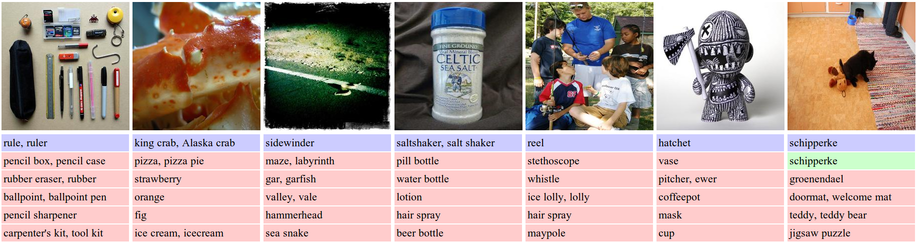
\includegraphics[width=1\textwidth]{example_errors.png}
    \caption{Representative validation images that highlight common sources of error. For each image, we display the ground truth in blue, and top 5 predictions from GoogLeNet follow (red = wrong, green = right). GoogLeNet predictions on the validation set images were graciously provided by members of the GoogLeNet team. From left to right: Images that contain multiple objects, images of extreme closeups and uncharacteristic views, images with filters, images that significantly benefit from the ability to read text, images that contain very small and thin objects, images with abstract representations, and example of a fine-grained image that GoogLeNet correctly identifies but a human would have significant difficulty with.}
    \label{fig:example_errors}
\end{figure*}

\subsubsection{Analysis of human and computer errors on large-scale image classification} 

We manually inspected both human and GoogLeNet errors to gain an understanding of common error types and how they compare. For purposes of this section, we only discuss results based on the larger sample of 1500 images that were labeled by annotator A1. Examples of representative mistakes are in Figure \ref{fig:example_errors}. The analysis and insights below were derived specifically from GoogLeNet predictions, but we suspect that many of the same errors may be present in other methods.

\paragraph{Types of errors in both computer and human annotations:}

\begin{enumerate}
\item \textbf{Multiple objects.} Both GoogLeNet and humans struggle with images that contain multiple ILSVRC classes (usually many more than five), with little indication of which object is the focus of the image. This error is only present in the Classification setting, since every image is constrained to have exactly one correct label. In total, we attribute 24 ($24\%$) of GoogLeNet errors and 12 ($16\%$) of human errors to this category. It is worth noting that humans can have a slight advantage in this error type, since it can sometimes be easy to identify the most salient object in the image.

\item \textbf{Incorrect annotations.} We found that approximately 5 out of 1500 images ($0.3\%$) were incorrectly annotated in the ground truth. This introduces an approximately equal number of errors for both humans and GoogLeNet.
\end{enumerate}

\paragraph{Types of errors that the computer is more susceptible to than the human:}

\begin{enumerate}
\item \textbf{Object small or thin.} GoogLeNet struggles with recognizing objects that are very small or thin in the image, even if that object is the only object present. Examples of this include an image of a standing person wearing sunglasses, a person holding a quill in their hand, or a small ant on a stem of a flower. We estimate that approximately 22 ($21\%$) of GoogLeNet errors fall into this category, while none of the human errors do. In other words, in our sample of images, no image was mislabeled by a human because they were unable to identify a very small or thin object. This discrepancy can be attributed to the fact that a human can very effectively leverage context and affordances to accurately infer the identity of small objects (for example, a few barely visible feathers near person's hand as very likely belonging to a mostly occluded quill).

\item \textbf{Image filters.} Many people enhance their photos with filters that distort the contrast and color distributions of the image. We found that 13 ($13\%$) of the images that GoogLeNet incorrectly classified contained a filter. Thus, we posit that GoogLeNet is not very robust to these distortions. In comparison, only one image among the human errors contained a filter, but we do not attribute the source of the error to the filter.

\item \textbf{Abstract representations}. GoogLeNet struggles with images that depict objects of interest in an abstract form, such as 3D-rendered images, paintings, sketches, plush toys, or statues. An example is the abstract shape of a bow drawn with a light source in night photography, a 3D-rendered robotic scorpion, or a shadow on the ground, of a child on a swing. We attribute approximately 6 ($6\%$) of GoogLeNet errors to this type of error and believe that humans are significantly more robust, with no such errors seen in our sample.

\item \textbf{Miscellaneous sources.} Additional sources of error that occur relatively infrequently include extreme closeups of parts of an object, unconventional viewpoints such as a rotated image, images that can significantly benefit from the ability to read text (e.g. a featureless container identifying itself as ``face powder''), objects with heavy occlusions, and images that depict a collage of multiple images. In general, we found that humans are more robust to all of these types of error.
\end{enumerate}

\paragraph{Types of errors that the human is more susceptible to than the computer:}

\begin{enumerate}

\item \textbf{Fine-grained recognition.} We found that humans are noticeably worse at fine-grained recognition (e.g. dogs, monkeys, snakes, birds), even when they are in clear view. To understand the difficulty, consider that there are more than 120 species of dogs in the dataset. We estimate that 28 ($37\%$) of the human errors fall into this category, while only 7 ($7\%$) of GoogLeNet errors do.

\item \textbf{Class unawareness.} The annotator may sometimes be unaware of the ground truth class present as a label option. When pointed out as an ILSVRC class, it is usually clear that the label applies to the image. These errors get progressively less frequent as the annotator becomes more familiar with ILSVRC classes. Approximately 18 ($24\%$) of the human errors fall into this category.

\item \textbf{Insufficient training data.} Recall that the annotator is only presented with 13 examples of a class under every category name. However, 13 images are not always enough to adequately convey the allowed class variations. For example, a brown dog can be incorrectly dismissed as a ``Kelpie'' if all examples of a ``Kelpie'' feature a dog with black coat. However, if more than 13 images were listed it would have become clear that a ``Kelpie'' may have brown coat. Approximately 4 ($5\%$) of human errors fall into this category.

\end{enumerate}

\subsubsection{Conclusions from human image classification experiments} 

We investigated the performance of trained human annotators on a sample of 1500 ILSVRC test set images. Our results indicate that a trained human annotator is capable of outperforming the best model (GoogLeNet) by approximately $1.7\%$ ($p = 0.022$). 

We expect that some sources of error may be relatively easily eliminated (e.g. robustness to filters, rotations, collages, effectively reasoning over multiple scales), while others may prove more elusive (e.g. identifying abstract representations of objects). On the other hand, a large majority of human errors come from fine-grained categories and class unawareness. We expect that the former can be significantly reduced with fine-grained expert annotators, while the latter could be reduced with more practice and greater familiarity with ILSVRC classes. Our results also hint that human errors are not strongly correlated and that human ensembles may further reduce human error rate.

It is clear that humans will soon outperform state-of-the-art ILSVRC image classification models only by use of significant effort, expertise, and time. One interesting follow-up question for future investigation is how computer-level accuracy compares with human-level accuracy on more complex image understanding tasks.






